\setcounter{section}{-1}
\Section{Введение}

\noindent
\begin{minipage}[c]{0.3\textwidth}
  \centering
  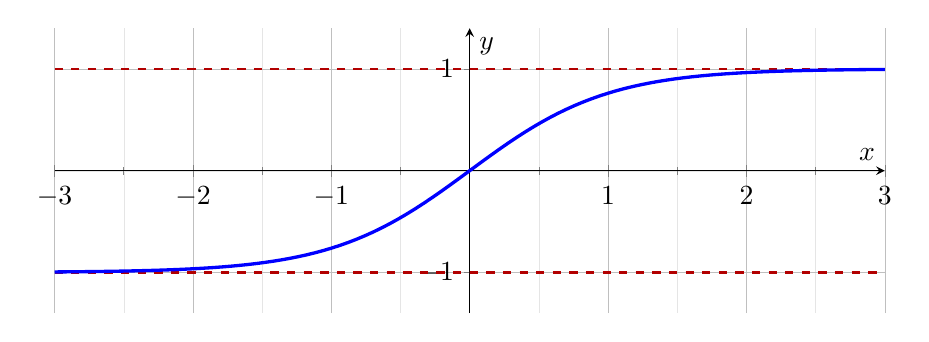
\begin{tikzpicture}
    \begin{axis}[
      width=\textwidth,
      height=5.2cm,
      axis lines=middle,
      xlabel={$x$},
      ylabel={$y$},
      xmin=-3, xmax=3,
      ymin=-1.4, ymax=1.4,
      ytick={-1, 1}, 
      grid=both,
      minor tick num=1,
      grid style={line width=.1pt, draw=gray!20},
      major grid style={line width=.2pt, draw=gray!50}
    ]
      \addplot[domain=-3:3, dashed, red!70!black, thick] {1};
      \addplot[domain=-3:3, dashed, red!70!black, thick] {-1};
      \addplot[domain=-3:3, samples=100, very thick, blue] {tanh(x)};
    \end{axis}
  \end{tikzpicture}
\end{minipage}%
\hfill
\begin{minipage}[c]{0.7\textwidth}
  Рассмотрим функцию $\th{x} \in C^{\infty} (\R)$. Известно, что её можно представить в виде $\th{x} = \sum_{n = 0}^{\infty} a_n x^n$. Если поставить задачу нахождения радиуса сходимости данного ряда, то решить её методами, известными нам из прошлых семестров, невозможно. Вообще говоря, радиус сходимости $R_{\text{сх}} = \frac{\pi}{2}$. Чтобы его найти, нужно выйти в комплексную плоскость.
\end{minipage}

\Section{Комплексные числа. Алгебраическая и тригономентрическая формы}

Рассмотрим пары чисел $z = (x, y) \in \R^2$. Для удобства отметим, что $z_i = (x_i, y_i)$. Введём основные операции над парами чисел.
\begin{enumerate}
    \item Сложение и разность двух пар чисел: $z_1 \pm z_2 = (x_1 \pm x_2, y_1 \pm y_2)$;
    \item \label{1:criterion_equality} Проверка равенства двух пар чисел: $\left[z_1 = z_2\right] \iff \{\left[x_1 = x_2\right] \& \left[y_1 = y_2\right]\}$;
    \item Модуль пар чисел: $|z| = \left\|(x, y)\right\| = \sqrt{x^2 + y ^2}$
    \item Произведение пар чисел: $z_1 \cdot z_2 = (x_1, y_1) \cdot (x_2, y_2) = (x_1x_2 - y_1y_2, x_1y_2 + x_2y_1)$. \textit{Далее знак произведения может опускаться}.
\end{enumerate}

Отметим свойства, следующие из введённых операций:
\begin{properties}
    \item $z_1(z_2z_3) = (z_1z_2)z_3$;
    \item $z_1z_2 = z_2z_1$;
    \item $z \cdot (1, 0) = z$;
    \item $z_1(z_2+z_3) = z_1 z_2 + z_1 z_3$;
    \item $\forall z_2, \, \forall z_1 \neq (0, 0) \quad \exists! z_3 \colon z_3 z_1 = z_2$. При этом $z_3 = \frac{z_2}{z_1}$.
    \item $||z_2| - |z_1|| \le |z_1 \pm z_2| \le |z_1| + |z_2|$
\end{properties}
\begin{proof}
    Свойства 1-4 доказываются подстановкой $z = (x, y)$. Свойство 6 доказывается аналогично неравенству треугольника из прошлых семестров. Докажем свойство 5:

    $(x_1, y_1) (x_3, y_3) = (x_2, y_2) \iff (x_1 x_3 - y_1 y_3, x_1 y_3 + x_3 y_1) = (x_2, y_2)$. Из критерия равенства двух пар чисел (\ref{1:criterion_equality}) следует система уравнений:
    \[\begin{bmatrix}
        x_1 & -y_1 \\
        y_1 & x_1
    \end{bmatrix}
    \begin{bmatrix}
        x_3 \\
        y_3
    \end{bmatrix}
    =
    A \cdot 
    \begin{bmatrix}
        x_3 \\
        y_3
    \end{bmatrix}
    =
    \begin{bmatrix}
        x_2 \\
        y_2
    \end{bmatrix}.\]

    Так как $z_1 \neq (0, 0) \implies \det{A} = x_1^2 + y_1^2 \neq 0 \implies \exists! z_3 - \text{решение системы} $.
\end{proof}

\begin{definition}
    \textit{Полем комплексных чисел $\Co$} назовём множество $\R^2$ с введёнными выше операциями.
\end{definition}

Также отметим, что $(x_1, 0) + (x_2, 0) = (x_1 + x_2, 0)$ и $(x_1, 0) (x_2, 0) = (x_1 x_2, 0)$. То есть в поле $\Co$ существует подполе, изоморфное полю действительных чисел $(x, 0) \sim x$.

\begin{definition}
    \textit{Мнимой единицей $i$} назовём комплексное число вида $(0, 1)$.
\end{definition}

Заметим, что любое комплексное число $z$ можно представить в виде $z = (x, y) = (x, 0) + (1, 0) (y, 0)$. Отсюда следует определение алгебраической формы записи комплексного числа.

\begin{definition}
    \textit{Алгебраической формой записи комплексного числа $z$} назовём запись вида $z = z + i y$.
\end{definition}

Аналогично записи в форме пары чисел, можно ввести критерий равенства двух комплексных чисел в арифметической форме: \[\left[z_1 = z_2\right] \iff \left[x_1 = x_2\right] \& \left[y_1 = y_2\right].\]

\begin{definition}
    \textit{Действительной частью числа $z$} назовём $\re{z} = x$. \textit{Мнимой частью числа $z$} назовём $\im{z} = y$.
\end{definition}

\noindent
\begin{minipage}[c]{0.4\textwidth}
  \centering
  \shorthandoff{"}
  \begin{tikzpicture}[>=stealth, scale=1.1]
    % Координатные оси
    \draw[->, thick] (-0.5, 0) -- (3.8, 0) node[right] {$\text{x}$};
    \draw[->, thick] (0, -0.5) -- (0, 2.8) node[above] {$\text{y}$};

    % Точки
    \coordinate (O) at (0,0);
    \coordinate (X) at (3,0);
    \coordinate (Z) at (3,2);

    % Проекции
    \draw[dashed, gray] (3,0) -- (3,2) node[below, pos=0, black] {$x$};
    \draw[dashed, gray] (0,2) -- (3,2) node[left, pos=0, black] {$y$};

    % Вектор r
    \draw[->, very thick, blue] (O) -- (Z) node[midway, above left, black] {$r$};

    % Точка z
    \filldraw[blue] (Z) circle (2pt) node[above right, black] {$z = x + iy$};

    % Угол phi
    \pic [draw, ->, "$\phi$", angle radius=0.9cm, angle eccentricity=1.3] 
      {angle = X--O--Z};
  \end{tikzpicture}
  \shorthandon{"}
\end{minipage}%
\hfill
\begin{minipage}[c]{0.6\textwidth}
  На рисунке:
  \begin{itemize}
    \item $r = |z| = \sqrt{x^2 + y^2}$ — модуль комплексного числа;
    \item $\phi = \arg z$ — аргумент комплексного числа, определённый с точностью до $2\pi k, k \in \Z$.
  \end{itemize}
\end{minipage}

\begin{definition}
    Легко заметить, что $x = r\cos{\phi}$, $y = r\sin{\phi}$. С помощью введённых обозначений, комплексное число $z$ можно переписать в виде: $z = r(\cos{\phi} + i\sin{\phi})$. \textit{Такую форму записи комплексного числа будем называть тригонометрической}.
\end{definition}

Критерий равенства двух комплексных чисел в тригонометрической форме $z_1 = r_1(\cos{\phi_1} + i\sin{\phi_1})$ и $z_2 = r_2(\cos{\phi_2} + i\sin{\phi_2})$ выглядит следующим образом: \[z_1 = z_2 \iff \left[r_1 = r_2\right] \& \left[\exists k \in \Z \colon \phi_2 = \phi_1 + 2\pi k\right]\]

\begin{example}
\par\noindent

\begin{minipage}[c]{0.3\textwidth}
  \centering
  \shorthandoff{"}
  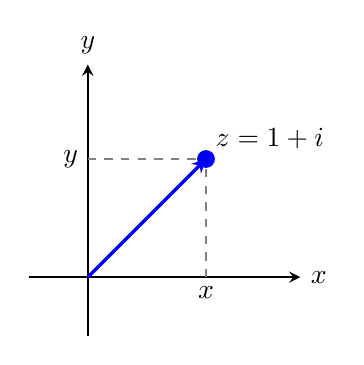
\begin{tikzpicture}[>=stealth, scale=1.5]
    % Координатные оси
    \draw[->, thick] (-0.5, 0) -- (1.8, 0) node[right] {$\text{x}$};
    \draw[->, thick] (0, -0.5) -- (0, 1.8) node[above] {$\text{y}$};

    % Точки
    \coordinate (O) at (0,0);
    \coordinate (X) at (3,0);
    \coordinate (Z) at (1,1);

    % Проекции
    \draw[dashed, gray] (1,0) -- (1,1) node[below, pos=0, black] {$x$};
    \draw[dashed, gray] (0,1) -- (1,1) node[left, pos=0, black] {$y$};

    % Вектор r
    \draw[->, very thick, blue] (O) -- (Z) node[midway, above left, black] {};

    % Точка z
    \filldraw[blue] (Z) circle (2pt) node[above right, black] {$z = 1 + i$};
  \end{tikzpicture}
  \shorthandon{"}
\end{minipage}%
\hfill
\begin{minipage}[c]{0.65\textwidth}
    Число $z$ можно записать как: $1 + i = \sqrt{2}(\cos{\dfrac{\pi}{4} + i\sin{\dfrac{\pi}{4}}})$
\end{minipage}
\end{example}

\Section{Функции комплексного переменного. Элементарные функции}

Функции комплексного переменного будем обозначать следующим образом: $w = f(z) \ w, z\in\Co$. Введём две основные элементарные функции:
\begin{enumerate}
    \item Многочлены $P(z) = a_n z^n + \dots + a_1 z + a_0, \ a_i \in \Co \forall i = \overline{0,n}$;
    \item Экспонента $f(z) = e^z = e^x(\cos{y} + i\sin{y})$.
\end{enumerate}

\begin{note}\label{2:criterion_zero}
    Критерий нуля: $w = 0 \iff |w| = 0$.
\end{note}

Отметим свойства экспоненты:
\begin{properties}
    \item $e^{x+i\cdot 0} = e^x$, \textit{т. е. экспонента комплексного числа без мнимой части равна экспоненте его действительной части};
    \item \label{2:exp_neq_0}$\forall z \in \Co \mapsto e^z \neq 0$;
    \item Периодичность: $e^z$ является периодической функцией, при этом её периодами являются $T = 2\pi k i, \ k\in \Z$; других периодов нет;
    \item \label{2:exp_mult} $e^{z_1} e^{z_2} = e^{z_1 + z_2} $
    \item \label{2:exp_inv}  $\forall z \neq 0 \mapsto (z^{-1})^n = (z^n)^{-1}, \  \forall n \in \N$
\end{properties}
\begin{proof}
    Свойства 1-2, 5, а также первая часть свойства 3 доказываются подстановкой.

    Докажем отсутствие периодов другого вида у экспоненты (вторую часть свойства 3). Пусть период комплексной экспоненты равен $T = T_1 + i T_2$. Тогда $e^{z + T_1 + i T_2} = e^z$, в частности $e^{T_1 + i T_2} = 1 \implies |e^{T_1 + i T_2}| = e^{T_1} = 1 \implies T_1 = 0$. Тогда $e^{iT_2} = \cos{T_2} + i \sin{T_2} = 1 \overset{\ref{1:criterion_equality}}{\iff} \cos(T_2) = 1 \ \& \ \sin(T_2) = 0 \implies T_2 = 2 \pi k i, \ k \in \Z$.

    Докажем свойство 4:
\begin{align*}
e^{z_1} e^{z_2} 
  &= e^{x_1}(\cos y_1 + i\sin y_1) \cdot e^{x_2}(\cos y_2 + i\sin y_2) \\
  &= e^{x_1 + x_2} \Big( (\cos y_1 \cos y_2 - \sin y_1 \sin y_2) + i(\sin y_1 \cos y_2 + \cos y_1 \sin y_2) \Big) \\
  &= e^{x_1 + x_2} (\cos(y_1 + y_2) + i\sin(y_1 + y_2)) \\
  &= e^{z_1 + z_2}.
\end{align*}

\end{proof}

\begin{corollary}
    Из свойств \ref{2:exp_mult} и \ref{2:exp_inv} следует $(e^z)^n = e^{nz} \forall n \in \Z$
\end{corollary}

\begin{definition}
    \textit{Элементарная функция ---} любая функция, полученная из основных элементарных функций с помощью арифметических операций и суперпозиции. Примерами служат: $R(Z) = \dfrac{P(z)}{Q(z)}$, $\cos{z} = \dfrac{e^{iz} + e^{-iz}}{2}$, $\sin{z} = \dfrac{e^{iz} - e^{-iz}}{2i}$, $\ch{z} = \dfrac{e^{z} + e^{-z}}{2}$, $\sh{z} = \dfrac{e^{z} - e^{-z}}{2}$, $\tg{z} = -i\dfrac{e^{iz} - e^{-iz}}{e^{iz} + e^{-iz}}$, $th{z} = \dfrac{e^z - e^{-z}}{e^z + e^{-z}}$.
\end{definition}

\begin{note}
    Легко доказываются следующие равенства:
    \begin{itemize}
        \item $\ch{iz} = \cos{z}$;
        \item $\cos{iz} = \ch{z}$;
        \item $\sh{iz} = i\sin{z}$;
        \item $\sin{iz} = i\sh{z}$;
    \end{itemize}
\end{note}

\Section{Показательная форма комплексного числа}

Используя равенство $e^{i\phi} = \cos{\phi} + i\sin{\phi}$ и тригонометрическую форму записи комплексного числа можно получить показательную форму записи тригонометрического числа $z = re^{i\phi}$.
\begin{properties}
    \item $z_1z_2 = r_1r_2e^{i(\phi_1 + \phi_2)}$; 
    \item $\dfrac{z_2}{z_1} = \dfrac{r_2}{r_1}e^{i(\phi_2 - \phi_1)}$;
    \item \label{3:kriterion_equality}Критерий равенства двух чисел в показательной форме идентичен критерию равенства двух чисел в тригонометрической форме:\[z_1 = z_2 \iff \left[r_1 = r_2\right] \& \left[\exists k \in \Z \colon \phi_2 = \phi_1 + 2\pi k\right]\]
\end{properties}
\begin{corollary}
    Характерны следующие свойства комплексных чисел:
    \begin{enumerate}
        \item $|z_1 z_2| = |z_1||z_2|$;
        \item $|z^n| = |z|^n$;
        \item $\left|\dfrac{z_2}{z_1}\right| = \dfrac{|z_2|}{|z_1|}$;
        \item $\arg{z_1 z_2} = \arg{z_1} + \arg{z_2}$;
        \item $\arg{\dfrac{z_2}{z_1}} = \arg{z_2} - \arg{z_1}$;
    \end{enumerate}
\end{corollary}
\begin{definition}
    \textit{Главным значением аргумента комплексного числа $\arg_0{z}$} будем называть значение его аргумента, лежащее в пределах $(-\pi, \pi]$.
\end{definition}
\begin{example}
    $\arg_0{(1+i)} = \dfrac{\pi}{4}$, $\arg_0{(-1)} = \pi$
\end{example}

\Section{Многозначные функции. \texorpdfstring{$\Ln z$}{Ln z} и \texorpdfstring{$\sqrt[n]{z}$}{sqrt[n](z)}}

\begin{definition}
    \textit{Логарифмом комплексного числа $z$} назовём множество $\Ln{z} = \{w \in \Co \colon e^w = z\}$.
\end{definition}

Найдём логарифм комплексного числа в общем случае:

\begin{enumerate}
    \item $z = 0 \overset{\text{\ref{2:exp_neq_0}}}{\implies} \Ln 0 = \varnothing$;
    \item $z \neq 0 \implies z = |z|e^{i\arg_0{z}}$. Из \ref{3:kriterion_equality} комплексное число $w = u + iv$ является логарифмом комплексного числа $z$ тогда и только когда $e^u = |z| \ \& \ \exists k \in \N \colon v = \arg_0{z} + 2 \pi k$. Тогда $\Ln{z} = \{\ln{|z|} + i(\arg_0{z} + 2\pi k), \ k \in \N\}$.
\end{enumerate}

\begin{definition}
    \textit{Главным значением логарифма ненулевого комплексного числа $z$ $\ln_0{z}$} будем называть число $\ln_0{z} = \ln{z} + i \arg_0{z}$.
\end{definition}

\begin{example}
    $\ln_0{3 + 2i} = \dfrac{1}{2} \ln{13} + i\arctg{\dfrac{2}{3}}$.
\end{example}

\begin{definition}
    \textit{Корнем $n$-ой степени комплексного числа $z$} назовём множество $\sqrt[n]{z} = \{w \in \Co \colon w^n = z\}$.
\end{definition}

Найдём корень $n$-ой степени комплексного числа в общем случае:

\begin{enumerate}
    \item $z = 0 \implies w^n = 0 \overset{\ref{2:criterion_zero}}{\implies} |w^n| = 0 \implies |w|^n = 0 \implies |w| = 0 \overset{\ref{2:criterion_zero}}{\implies} w = 0$;
    \item $z \neq 0 \implies z = |z|e^{i\arg_0{z}}$. Из \ref{3:kriterion_equality} комплексное число $w = \rho e^{i\theta}$ является корнем $n$-ой степени комплексного числа $z$ тогда и только когда $\rho^n = |z| \ \& \ \exists k \in \N \colon n\theta = \arg_0{z} + 2 \pi k$. Тогда $w_k = \sqrt[n]{|z|}e^{i\dfrac{\arg_0{z} + 2 \pi k}{n}}, \ k \in \Z$. Вообще говоря, в какой-то момент значения аргумента $w$ начнут повторятся, если брать $k \in \Z$. Легко показать, что достаточно взять $k \in \overline{0, n-1}$.
\end{enumerate}

\begin{example}
    Найти все значения $\sqrt[7]{\sqrt{3} - i}$.

    \noindent
\begin{minipage}[c]{0.5\textwidth}
  \centering
  \shorthandoff{"}
  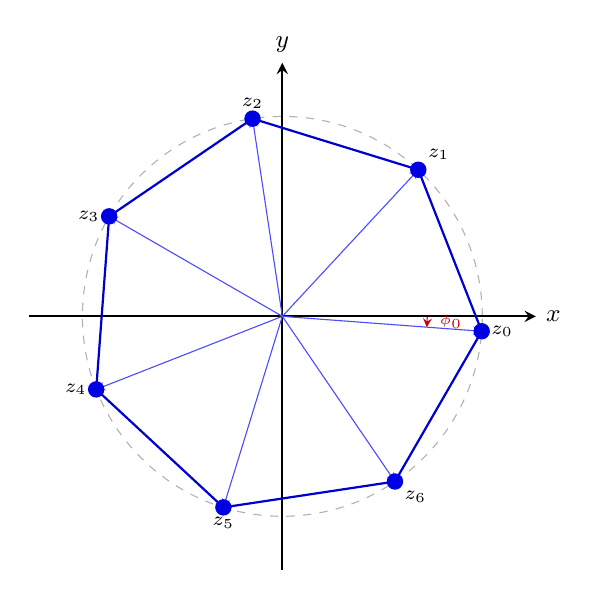
\begin{tikzpicture}[>=stealth, scale=2.3]
    \draw[dashed, gray!60] (0,0) circle (1.104);

    \draw[->, thick] (-1.4, 0) -- (1.4, 0) node[right] {\small $\text{x}$};
    \draw[->, thick] (0, -1.4) -- (0, 1.4) node[above] {\small $\text{y}$};

    \path ({-30/7 + 0*360/7}:1.104) coordinate (P0)
          ({-30/7 + 1*360/7}:1.104) coordinate (P1)
          ({-30/7 + 2*360/7}:1.104) coordinate (P2)
          ({-30/7 + 3*360/7}:1.104) coordinate (P3)
          ({-30/7 + 4*360/7}:1.104) coordinate (P4)
          ({-30/7 + 5*360/7}:1.104) coordinate (P5)
          ({-30/7 + 6*360/7}:1.104) coordinate (P6);

    \draw[thick, blue!80!black] 
      (P0) -- (P1) -- (P2) -- (P3) -- (P4) -- (P5) -- (P6) -- cycle;

    \foreach \i in {0,...,6} {
      \draw[->, thin, blue!70] (0,0) -- (P\i);
      \filldraw[blue!90!black] (P\i) circle (1.2pt);
    }

    \node[right, font=\scriptsize] at (P0) {$z_0$};
    \node[above right, font=\scriptsize] at (P1) {$z_1$};
    \node[above, font=\scriptsize] at (P2) {$z_2$};
    \node[left, font=\scriptsize] at (P3) {$z_3$};
    \node[left, font=\scriptsize] at (P4) {$z_4$};
    \node[below, font=\scriptsize] at (P5) {$z_5$};
    \node[below right, font=\scriptsize] at (P6) {$z_6$};

    \draw[->, red!80!black] (0.8,0) arc (0:{-30/7}:0.8) 
      node[midway, right=1pt, font=\tiny] {$\phi_0$};
  \end{tikzpicture}
  \shorthandon{"}
\end{minipage}
\hfill
\begin{minipage}[c]{0.45\textwidth}
    $n = 7$, $\arg_0{z} = -\dfrac{\pi}{6}$, $|z| = 2$, а значит значения корня задаются формулой:
      \[
      z_k = \sqrt[7]{2} \, e^{i \left( -\frac{\pi}{42} + \frac{2\pi k}{7} \right)}, \quad k = 0, \dots, 6.
      \]
      При этом  решения образуют правильный семиугольник.
\end{minipage}
\end{example}

\Section{Комплекснозначные функции вещественных переменных}

$w = f(t) = g(t) + ih(t), \ w \in \Co, t \in [a, b] \subset \R$ --- комплекснозначная функция вещественного переменного.

\begin{definition}
    $f \in C(t_0) \ \overset{def}{=} g, h \in C(t_0)$.
\end{definition}
\begin{definition}
    $f \in C^n[a, b] \ \overset{def}{=} g, h \in C^n[a, b]$.
\end{definition}
\begin{definition}
    $\int_{a}^{b} f(t)dt \overset{def}{=} \int_{a}^{b} g(t) dt + i\int_{a}^{b} h(t) dt$, при условии, что интегралы из правой части существуют.
\end{definition}